\chapter{Alignment with Human Preferences}
% Instruction Tuning and RLHF
% From Language Models to Assistants

This chapter includes recent topics on incorporating large-scale human feedback into language models.

\section{Instruction-Based Training Procedures}
 
Shortly after the advent of transformer-based language models, the pretraining-finetuning paradigm was shown to be an effective strategy for the great majority of NLP tasks. The ability of the pretraining stage to boost the performance of these models on downstream tasks led to the hypothesis that language models are unsupervised multitask learners \citep{radford2019language}. This idea suggests that models pretrained with a language modeling objective on large corpora are able to perform better because, during pretraining, these models implicitly learn a latent structure of the language that is useful to subsequently learn more effectively a task involving text.
While classic pretraining objectives leverage this ability of language models to implicitly learn information useful for multiple tasks, recent work proposed an explicit multi-task training paradigm that leverages the use of natural language instructions. We can identify two main approaches that follow this paradigm: instruction tuning and reinforcement learning from human feedback.

  \begin{figure}[ht]
    \centering
    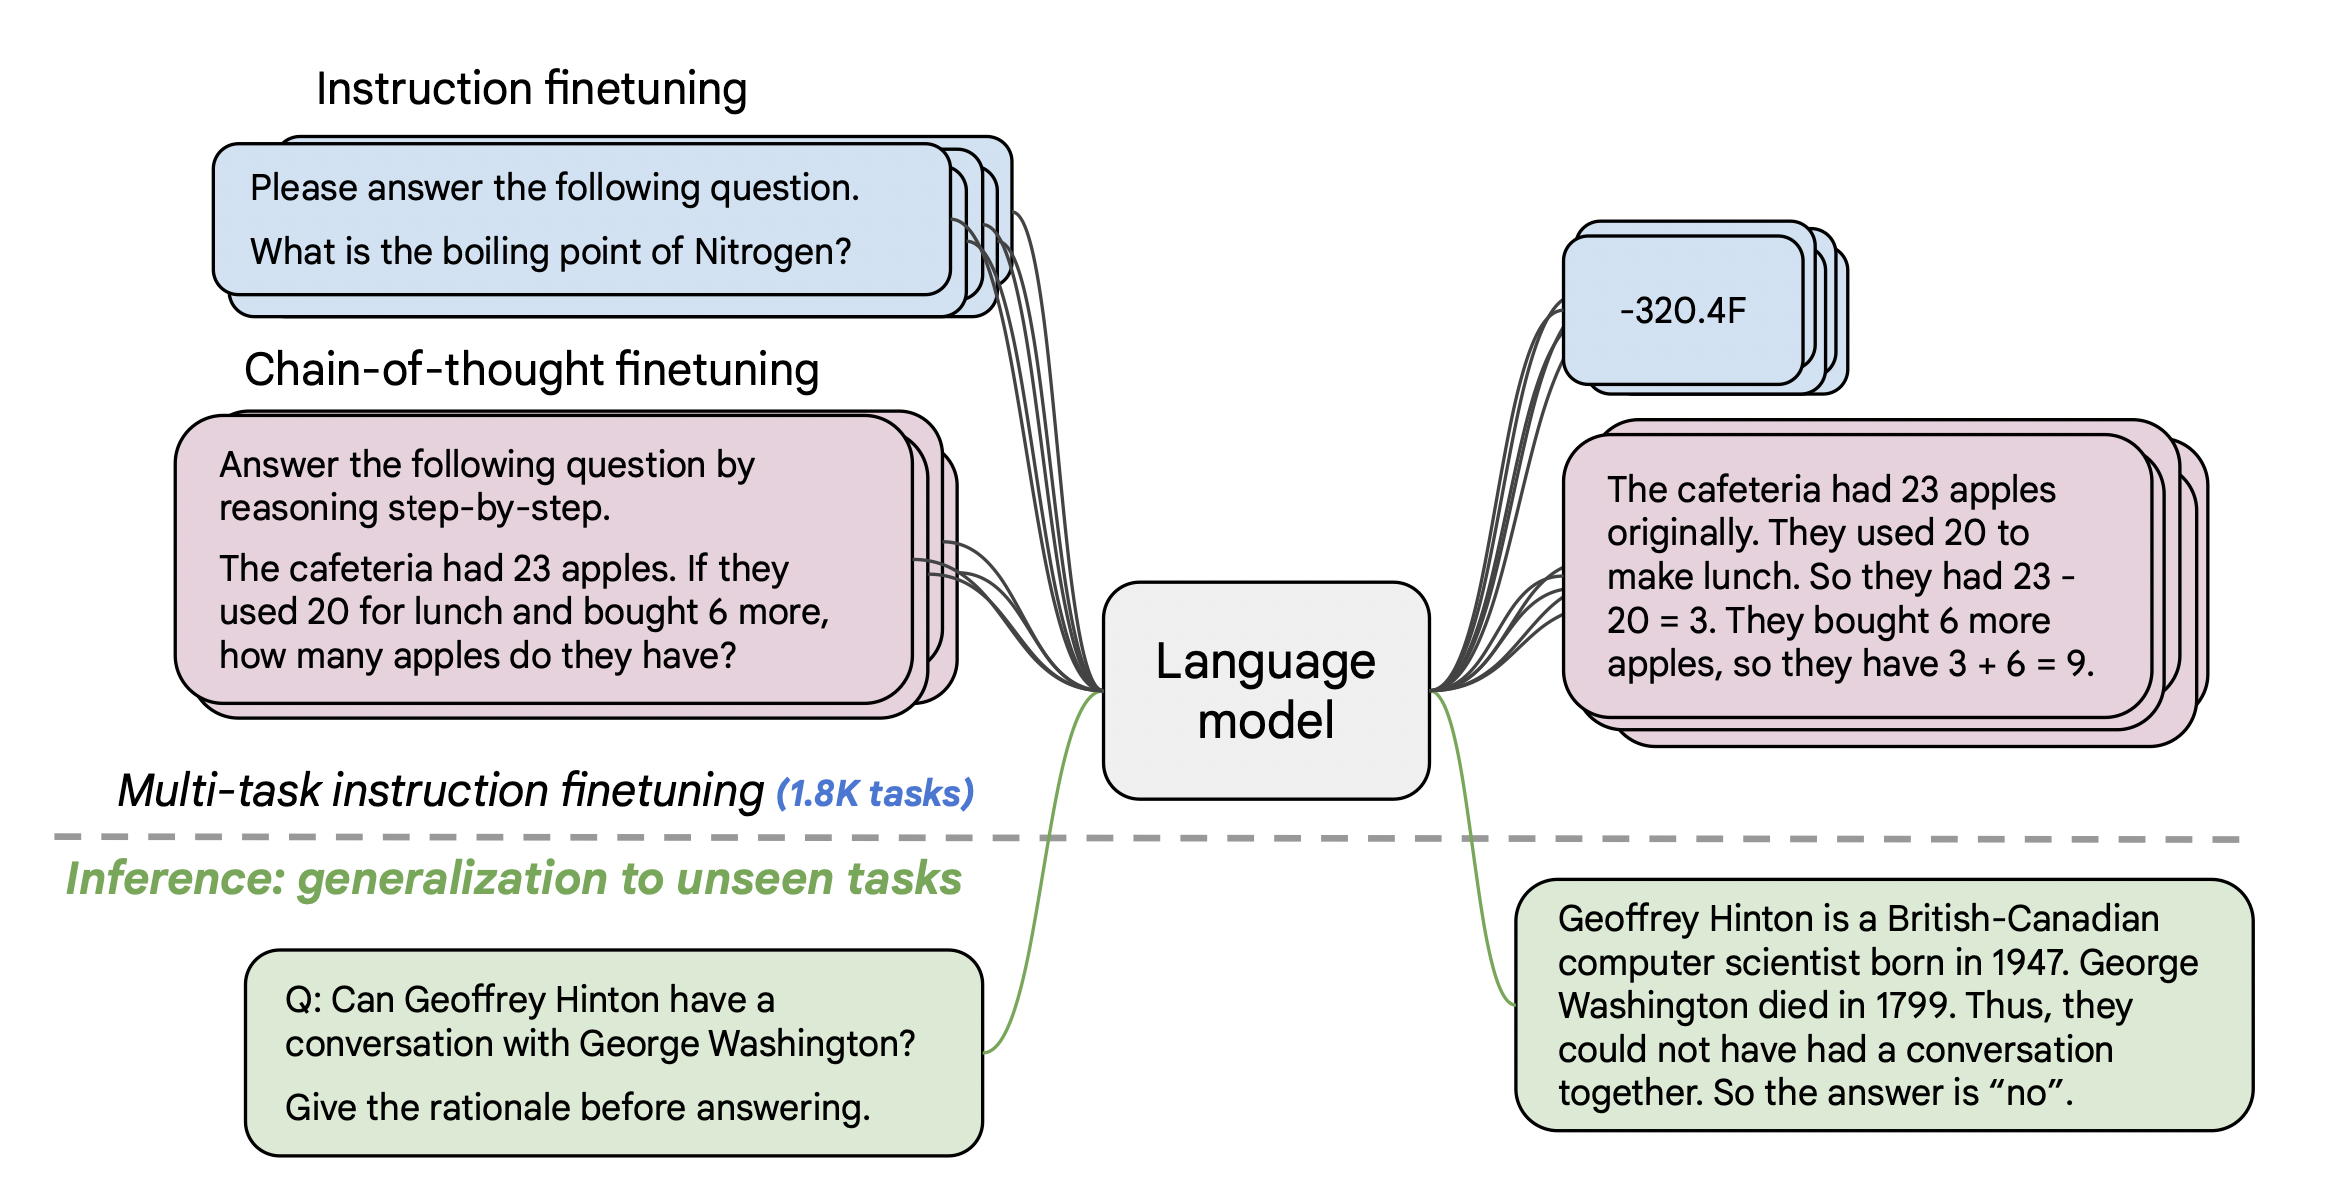
\includegraphics[width=\textwidth]{figures/additional_topics/flan.png}
    \caption{Example of instruction tuning. Taken from \citet{chung2022scaling}.
    \TODO{PDF screenshot instead of PNG.}
    }
    \label{fig:flan}
\end{figure}

 \subsection{Instruction Tuning}
Instruction tuning consists of finetuning language models on a collection of datasets described via instructions. The way these instructions are incorporated in the training procedure is simply by prepending to the model’s input a short description of the task that needs to be carried out (e.g., \textit{Is the sentiment of this movie review positive or negative?} or \textit{Translate the following sentence into Chinese}). This approach combines aspects of both pretrain-finetune and prompting paradigms to improve language models' responses to inference-time text interactions. 
By finetuning a pretrained language model on a mixture of NLP datasets expressed via natural language instructions, the models were shown to perform better on previously unseen tasks (process illustrated in Figure \ref{fig:flan}).

%\mrinmaya{Add results!}

%In instruction tuning, a pretrained language model is fine-tuned on a mixture of tens of NLP datasets expressed via natural language instructions.

An example of models trained using this procedure is the FLAN (Finetuned Language Net) family \citep{wei2022finetuned}. To evaluate the FLAN models’ ability to perform a specific task T (e.g., natural language inference), the model is instruction-tuned on a range of other NLP tasks such as commonsense reasoning, translation, and sentiment analysis. As this setup ensures that the FLAN model has not seen task T in instruction tuning, the model is evaluated on its ability to perform T in a zero-shot setting. FLAN models were shown to outperform larger LMs prompted with few shots (Figure \ref{fig:flan_results}). This approach was subsequently scaled to larger models (540B PaLM; \citealt{chowdhery2022palm}) and a larger number of tasks (1836) \citep{chung2022scaling}. This resulted in models with better generalization capabilities, improved reasoning abilities, and better behavior in open-ended zero-shot generation than non-instruction-tuned models. 


\begin{figure}[ht]
    \centering
    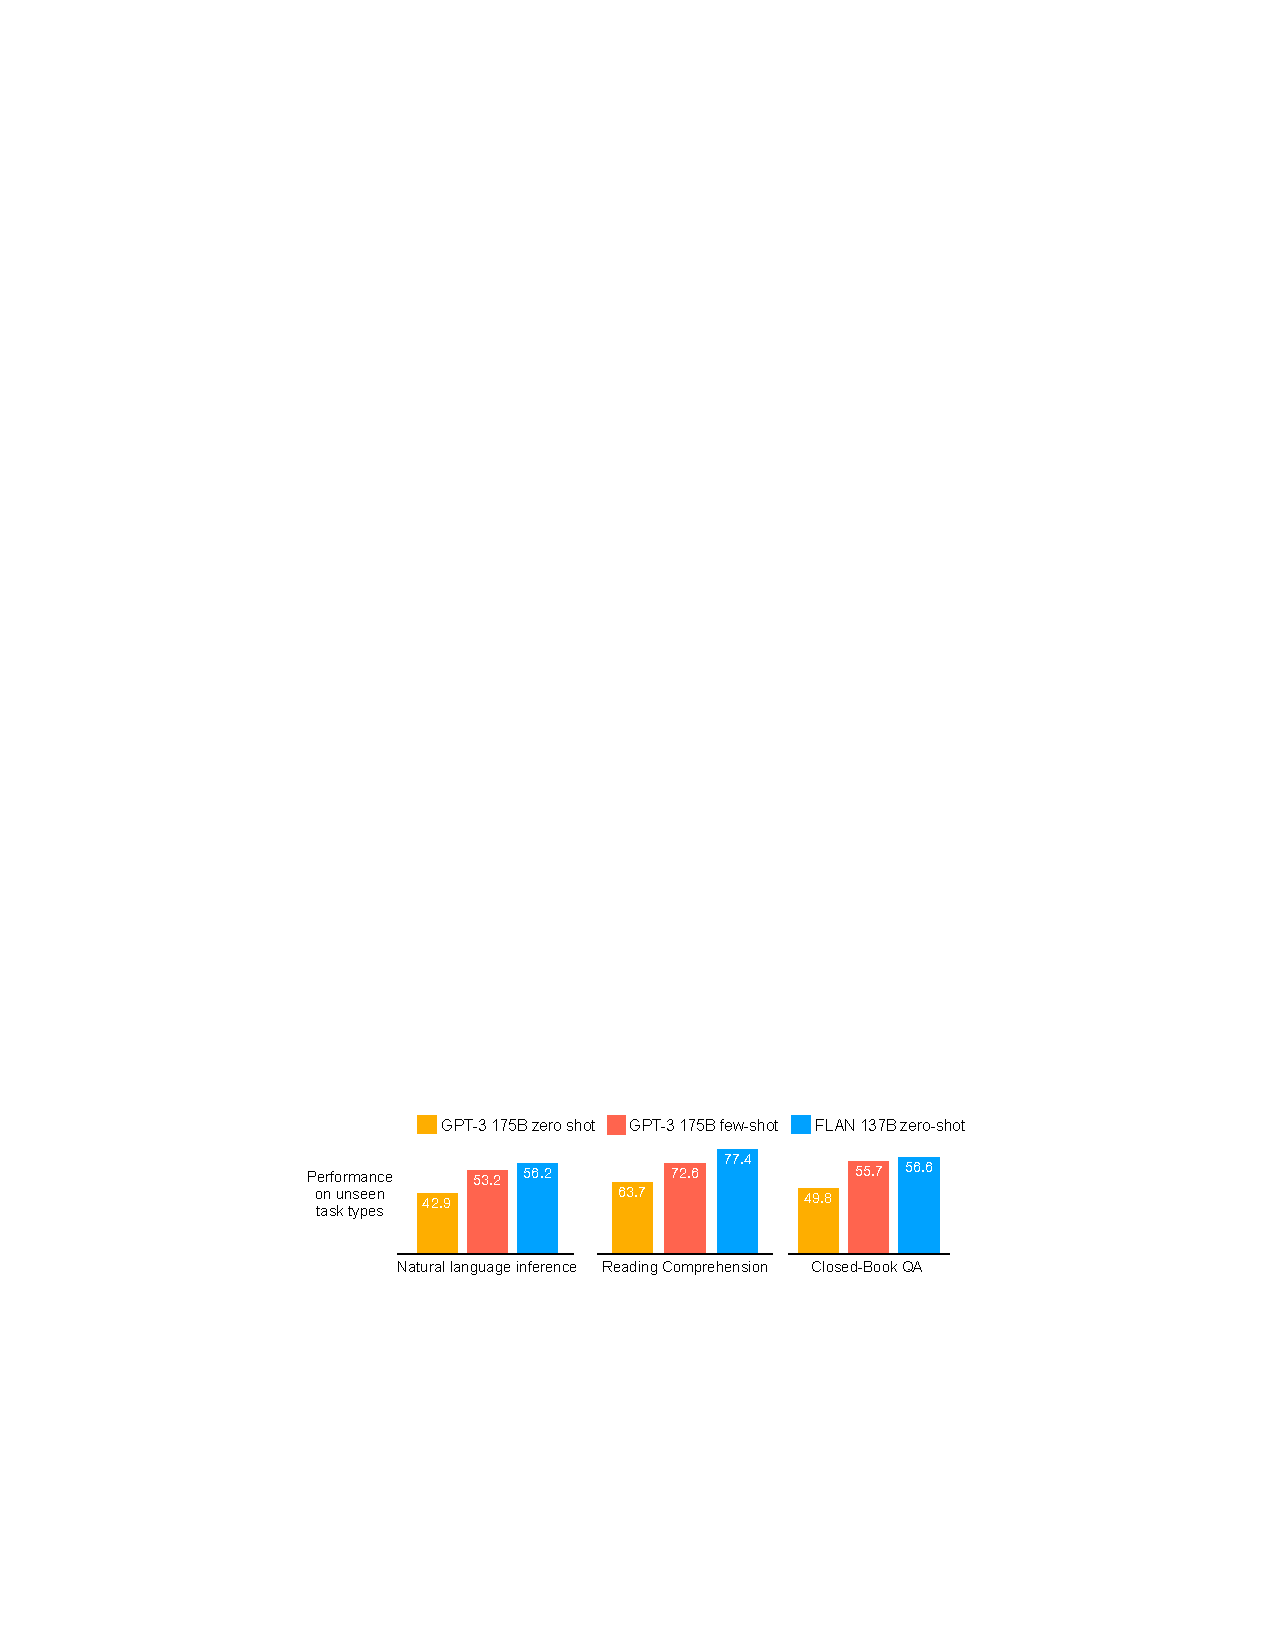
\includegraphics[width=\textwidth]{figures/additional_topics/flan_results.pdf}
    \caption{Performance of zero-shot FLAN, compared with zero-shot and few-shot GPT-3. Taken from \citet{wei2022finetuned}.
    }
    \label{fig:flan_results}
\end{figure}

%A concurrent work to FLAN that explores the same training paradigm is T0 …


\section{Reinforcement Learning from Human Feedback (RLHF)}

A different training approach that leverages human instructions is reinforcement learning from human feedback \citep{christiano2017deep}. Reinforcement learning (RL) is a branch of machine learning that focuses on how agents can learn to make decisions through interactions with an environment. In RL, an agent receives rewards or penalties based on its actions in the environment, and its objective is to maximize its cumulative reward over time. The reward function is a critical component of RL, as it specifies the goals and incentives for the agent. The agent's behavior is captured by a policy, which maps observations to actions. The goal of RL is to optimize the policy to maximize the expected cumulative reward.
The intuition behind RL from human feedback is to fit a reward function to the human's preferences while simultaneously training a policy to optimize the current predicted reward function.

In this setting, the agent that we are considering is a pre-trained language model that needs to be aligned with the user's intention. To this end, human preferences are used as a reward signal to train the model (process illustrated in Fig. \ref{fig:rlhf}). This procedure incorporates both explicit intentions such as following instructions and implicit intentions such as staying truthful, and not being biased, toxic, or otherwise harmful. RLHF consists of the following steps:

\begin{figure}[ht]
    \centering
    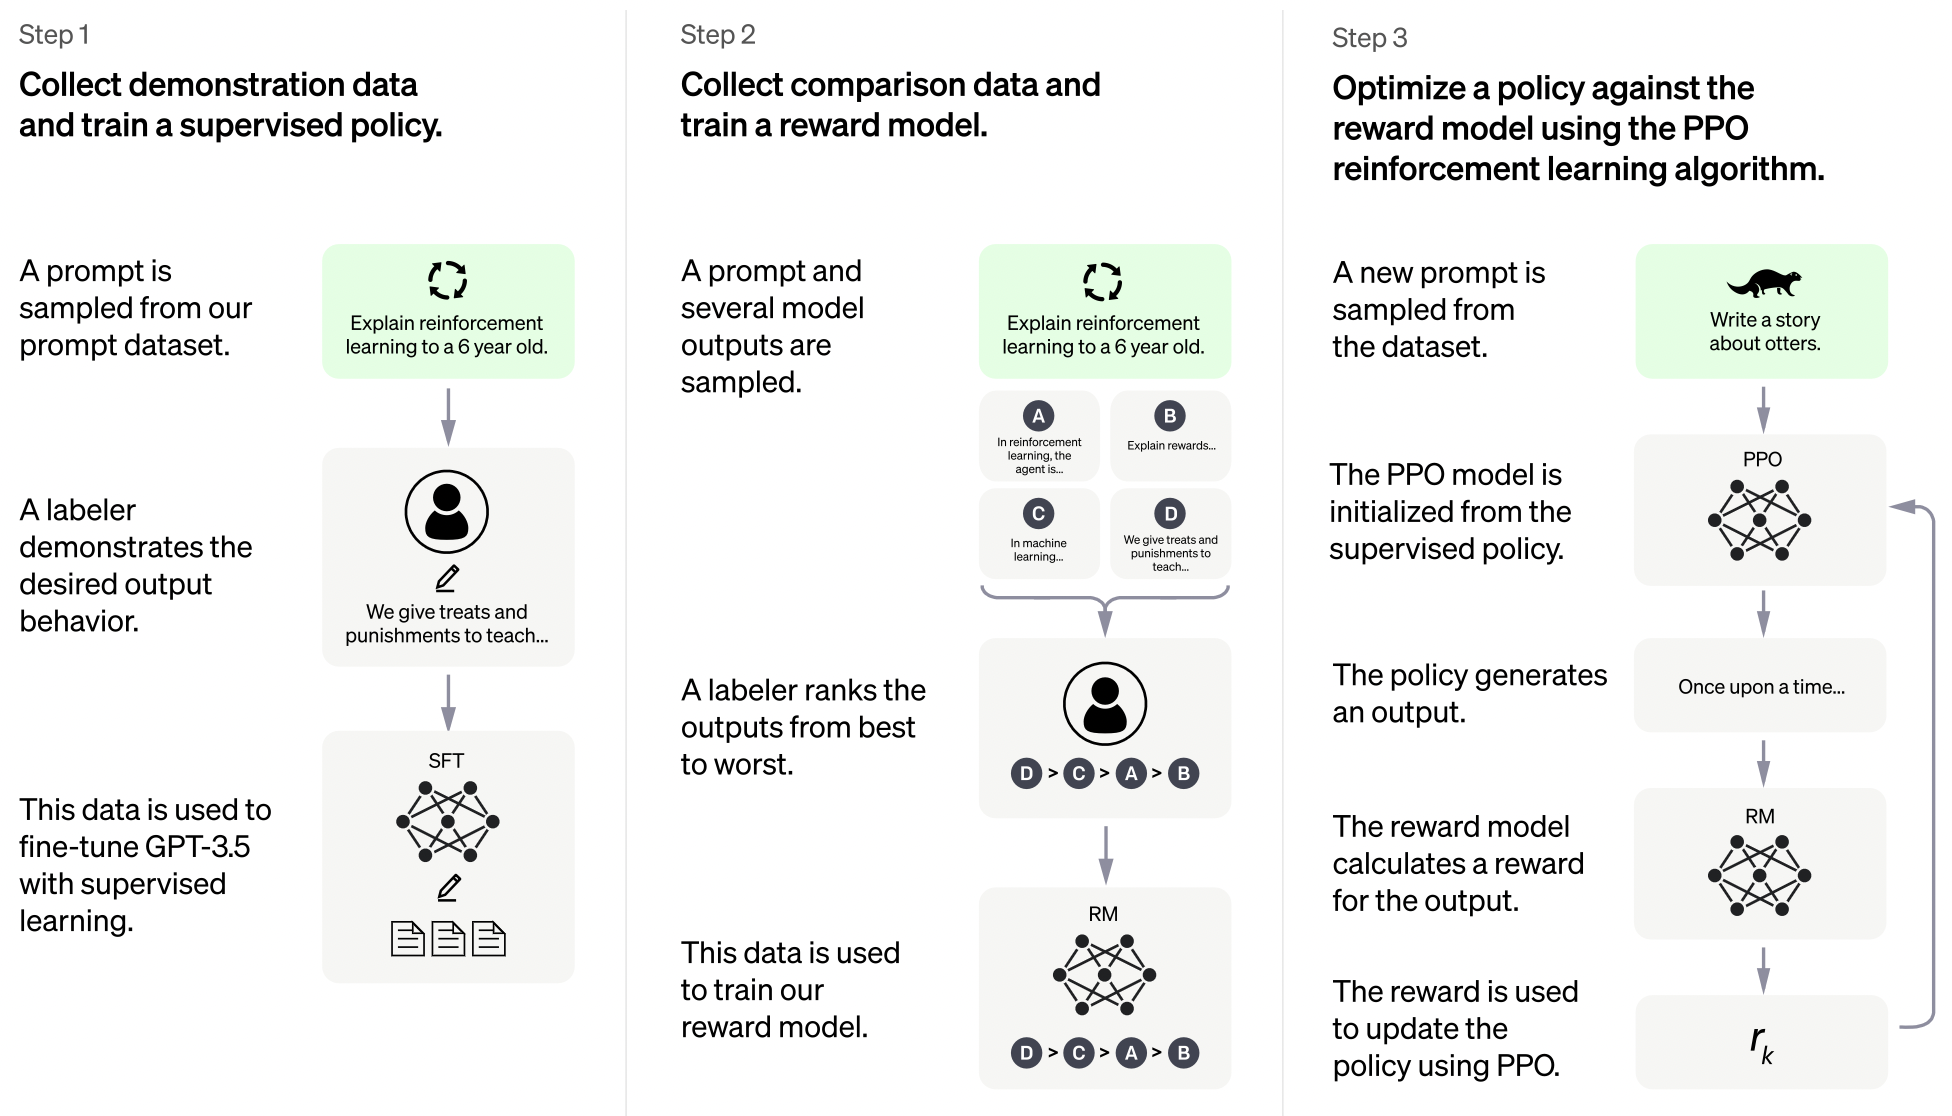
\includegraphics[width=0.8\textwidth]{figures/additional_topics/rlhf.png}
    \caption{ RLHF training procedure. Taken from \href{https://openai.com/blog/chatgpt}{openai.com/blog/chatgpt}.
    }
    \label{fig:rlhf}
\end{figure}

\begin{enumerate}
    \item Defining a distribution of prompts on which we want the model to produce aligned outputs.
    \item Constructing a dataset of human-written demonstrations and using it to train a supervised learning baseline model. These demonstrations represent the desired behavior on the input prompt distribution.
    \item Collecting a dataset $D$ of comparisons between outputs produced by the baseline model, where labelers indicate which output they prefer for a given input. A reward model is then trained to predict the human-preferred output. The loss function for the reward model $\theta_{RM}$ is:
    \begin{align}
     \mathcal{L}(\theta_{RM}) = - \frac{1}{\binom{K}{2}} E_{(x,y_w,y_l) \sim D} \big[ \log (\sigma (r_{\theta_{RM}} (x, y_w) -r_{\theta_{RM}} (x, y_l)))  \big],
    \end{align}
    where $r_{\theta}(x,y)$ is the scalar output of the reward model for prompt $x$ and completion $y$ with parameters $\theta$, $y_w$ is the preferred completion out of the pair of $y_w$ (winner over $y_l$), $y_l$ is dispreferred response, and $K$ is the number of ranked responses to prompt $x$ present in $D$.
    
    \item Using the output of the reward model as a scalar reward, fine-tune the supervised policy to optimize this reward using the proximal policy optimization (PPO) algorithm \citep{schulman2017proximal}. The objective function during this phase is:
    \begin{align}
        \text{obj}(\phi) = & E_{(x,y) \sim D_{\pi_{\phi}^{RL}}} \big[ r_{\theta_{RM}} (x, y) - \beta \log \frac{\pi_{\phi}^{RL}(y | x)}{\pi^{SFT}(y | x)} \big] + 
        \gamma E_{x \sim D_{\text{pretrain}}} \big [  \log (\pi_{\phi}^{RL} (x))\big ],
    \end{align}
    where $\pi_{\phi}^{RL}$ is the learned RL policy, $\pi^{SFT}$ is the supervised trained model, and $D_{\text{pretrain}}$ is the pretraining distribution. This objective combines a per-token Kullback-Leibler (KL) penalty from the supervised finetuning (SFT) model to mitigate over-optimization of the reward model, with a pretraining loss term. These terms are weighted by the parameters $\beta$ and $\gamma$, respectively.
\end{enumerate}

This procedure aligns the behavior of the language model to the stated preferences of a specific group of people. 

An example of models trained via RLHF is the InstructGPT series \citep{ouyangtraining}. For these models, the 175B-parameter GPT-3 is used as an SFT baseline model, while a smaller 6B model is used to model the reward. A human evaluation of the outputs produced by InstructGPT showed the efficacy of the RLHF technique: a set of labelers rated InstructGPT outputs favorably, compared to the predictions of the non-instruction-trained baseline, along multiple axes (e.g., compliance to the constraints in the prompt, lack of hallucinations, use of appropriate language). An aggregation of this result is displayed in Figure \ref{fig:instructgpt_res}. The same procedure was used to train the popular ChatGPT model, though with slight differences in the data collection setup.

\begin{figure}[ht]
    \centering
    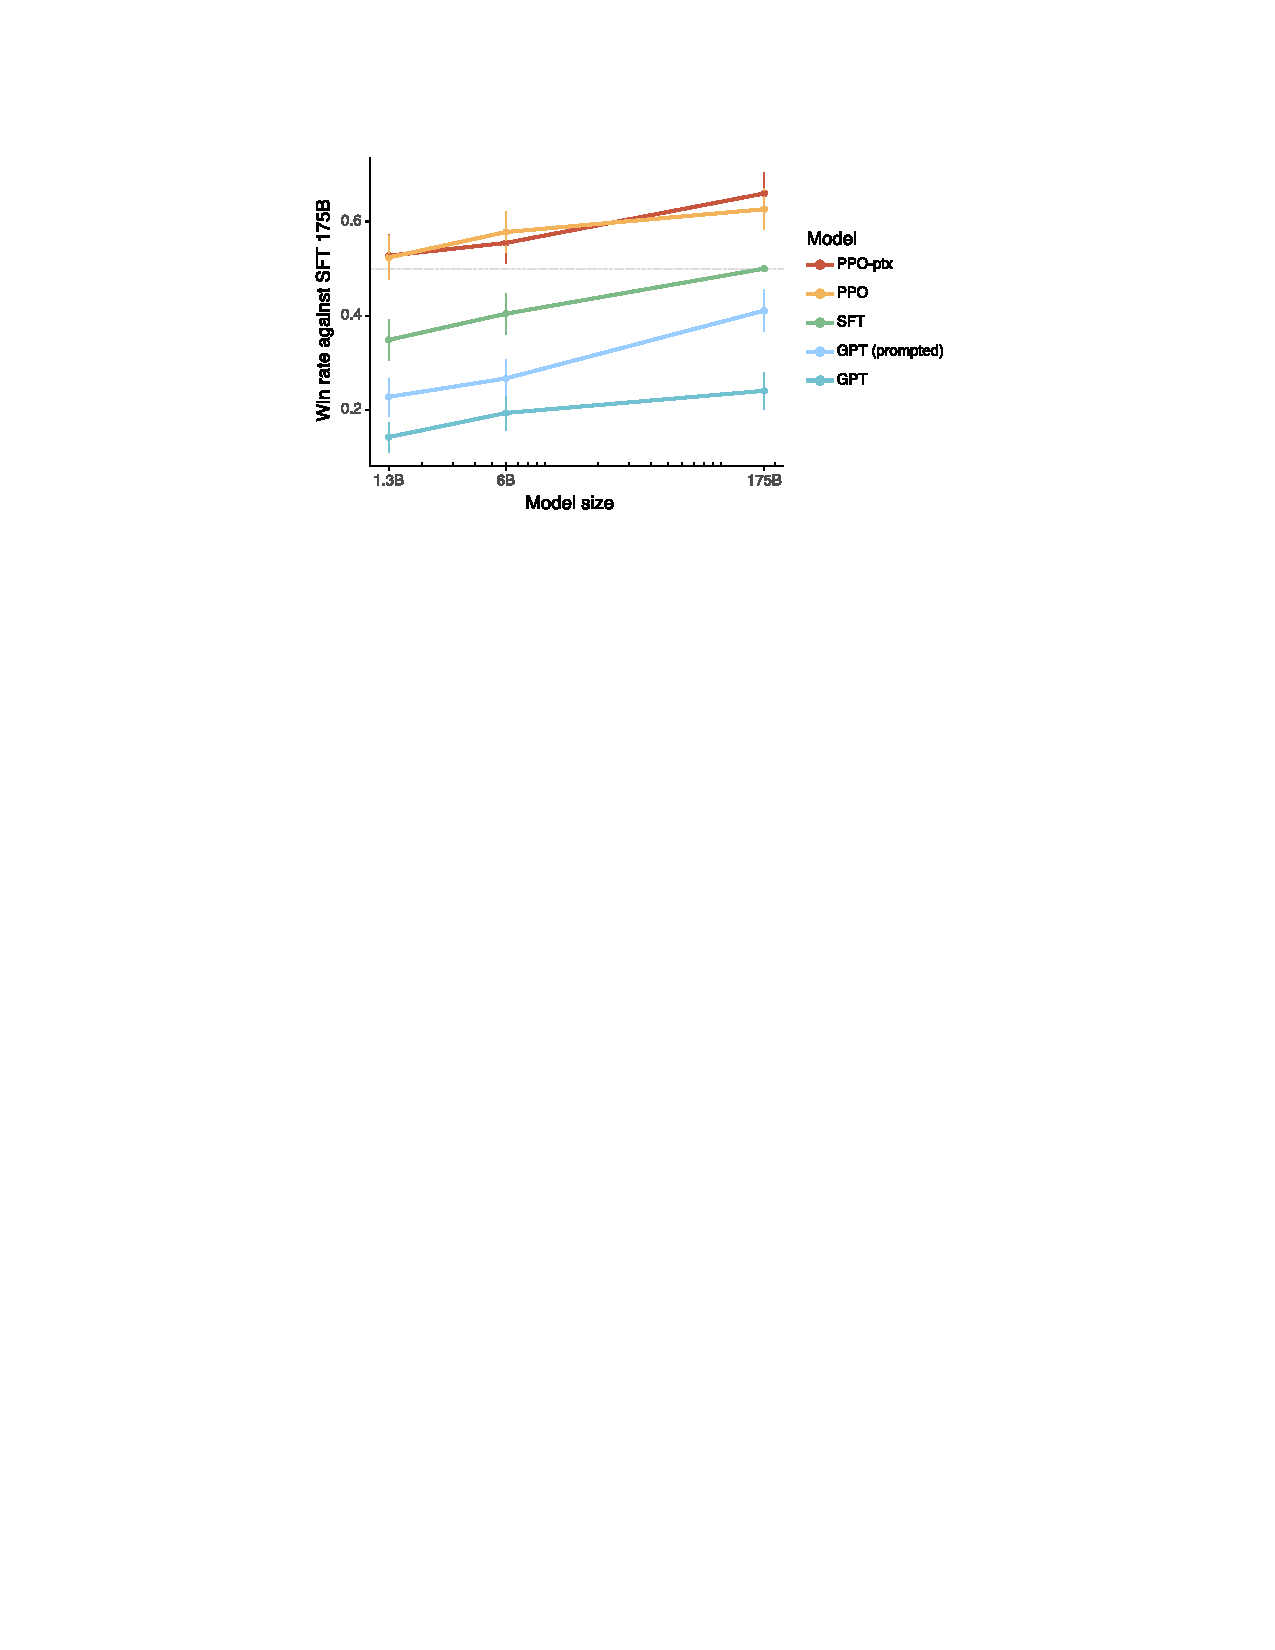
\includegraphics[width=0.75\textwidth]{figures/additional_topics/instructgpt_res.pdf}
    \caption{Multiple models evaluated by how often their outputs were preferred to those for the 175B SFT model, according to human evaluators. InstructGPT (PPO-ptx), as well as its variant without pretraining mix (PPO), significantly outperforms GPT-3.
    }
    \label{fig:instructgpt_res}
\end{figure}

%\mrinmaya{Add results from Instruct GPT? Particularly figure 1 in https://arxiv.org/pdf/2203.02155.pdf}

 

%  \newpage{}

% \mrinmaya{I will probably drop Calibration from this version of the course as we seem to have a lot of content. So no need to work on this. Sorry.}



\subsection{Direct Preference Optimization (DPO)}
The RLHF technique described in the previous chapter has several drawbacks. First, the training with RL objective is tricky, unstable, and sensitive to the choice of hyperparameters \citep{zheng2023secrets}. Secondly, the reward model is usually as large as the language model used making it computationally expensive to train and load into memory. 

\begin{figure}[ht]
    \centering
    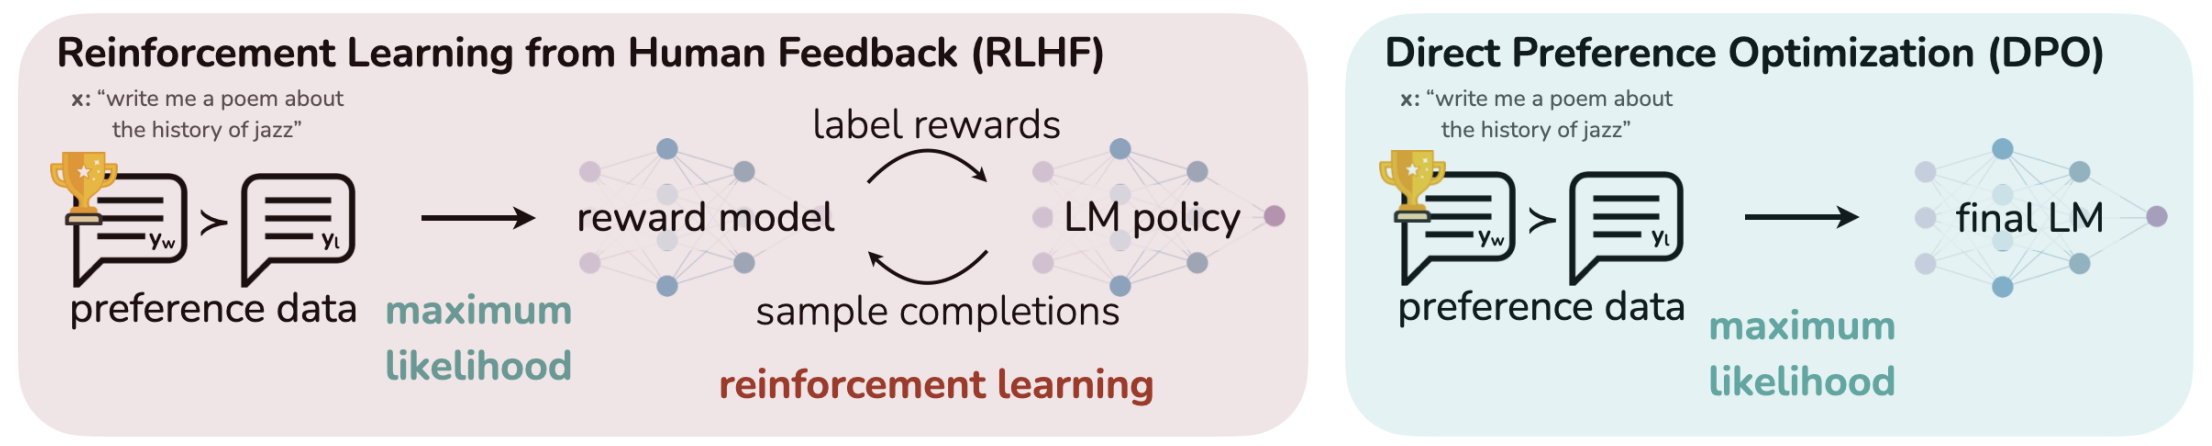
\includegraphics[width=1.0\textwidth]{figures/additional_topics/dpo.png}
    \caption{DPO optimizes for human preferences without using reward model or RL training loop. Taken from \citep{rafailov2024direct}.
    }
    \label{fig:dpo}
\end{figure}

Therefore, DPO \citep{rafailov2024direct} presents an alternative to RLHF which is simpler because it does not rely on any reward model nor use any RL loop. DPO directly fine-tunes language model weights to maximise the log-likelihood of preference data. DPO assumes the preference data can be modeled by the Bradley-Terry model \citep{bradley1952rank}: 
\begin{align}
p(\boldsymbol{y}_w \succ \boldsymbol{y}_l) = \sigma \big(r(\boldsymbol{x}, \boldsymbol{y}_w) - r(\boldsymbol{x}, \boldsymbol{y}_l) \big)
\end{align}
and framed as a binary classification minimizing the negative log-likelihood loss $\mathcal{L}(\theta_{RM})$.
%fine-tunes model weights to maximise log-likelihood of

DPO uses an observation that it is possible to extract the optimal policy that maximizes $\text{obj}(\phi)$ in the closed form \citep{peng2019advantage}:

\begin{align}
\pi^{\star} (\boldsymbol{y}|\boldsymbol{x})= \frac{1}{Z(\boldsymbol{x})} \pi^{\text{SFT}}(\boldsymbol{y}|\boldsymbol{x}) \exp\left(\frac{1}{\beta} r(\boldsymbol{x},\boldsymbol{y})\right),
\end{align}
where
\begin{align}
Z(x) = \sum_{y} \pi^{\text{SFT}}(\boldsymbol{y}|\boldsymbol{x}) \exp\left(\frac{1}{\beta} r(\boldsymbol{x},\boldsymbol{y})\right),
\end{align}
where the normalization term $Z(x)$ is a sum over all possible generated responses and is intractable to compute. However, if we write the reward as a function of $\pi^{*}$ by rearranging the terms,
\begin{align}
r\big(\boldsymbol{x}, \boldsymbol{y}) = \beta \log \frac{\pi^{\star} (\boldsymbol{y} \mid \boldsymbol{x})}{\pi^{\text{SFT}} (\boldsymbol{y} \mid \boldsymbol{x})} + \beta \log Z(\boldsymbol{x}),
\end{align}
assuming the preference data is modeled by Bradley--Terry model which depends on \textit{difference} in rewards between two completions, the intractable normalization term  $Z(x)$ cancels out when we take the difference. Therefore, the final DPO loss function directly optimizes language model parameters by minimizing the negative log-likelihood of the preference data:
\begin{align}
\mathcal{L}^{DPO}(\theta) = - E_{(x,y_w,y_l) \sim D} \big[ \log \sigma \big(\beta \log \frac{\pi^{\theta} (\boldsymbol{y_w} \mid \boldsymbol{x})}{\pi^{\text{SFT}} (\boldsymbol{y_w} \mid \boldsymbol{x})} - \beta \log \frac{\pi^{\theta} (\boldsymbol{y_l} \mid \boldsymbol{x})}{\pi^{\text{SFT}} (\boldsymbol{y_l} \mid \boldsymbol{x})}\big)  \big].
\end{align}
Notice that the model uses both preferred and dispreferred responses. The intuition behind this is to increase the likelihood of the preferred response and decrease the likelihood of the dispreferred response.


\begin{figure}[ht]
    \centering
    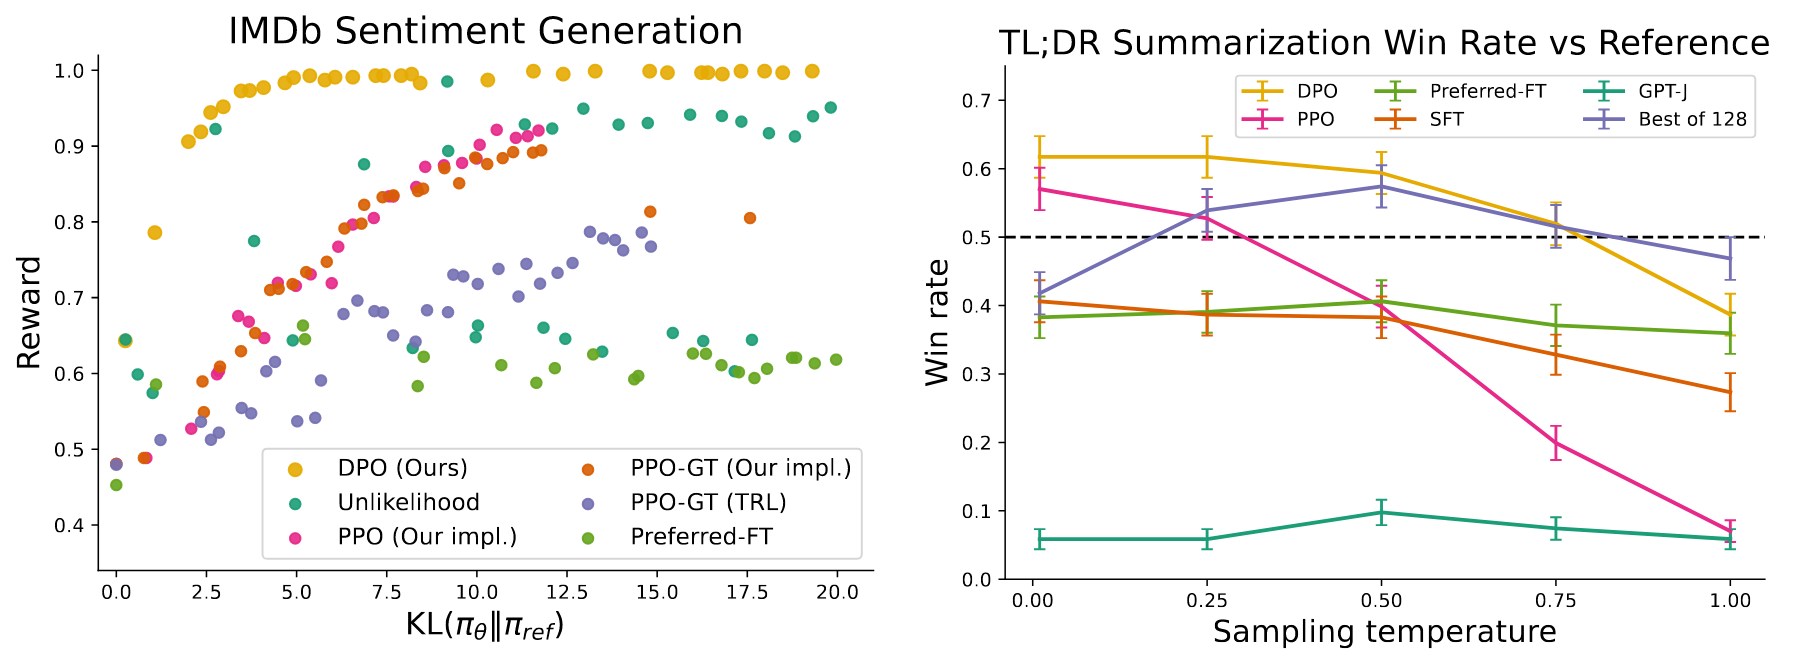
\includegraphics[width=1.0\textwidth]{figures/additional_topics/dpo-results.png}
    \caption{DPO provides the highest rewards for all KL values and outperforms other models in the summarization task. GPT-4 is used as an evaluator for win rate against baseline.
    }
    \label{fig:dpo-results}
\end{figure}

To summarize, compared to RL for human feedback, DPO has these properties:
\begin{itemize}
    \item Does not train an explicit reward model,
    \item Does not sample from the model to compute rewards but directly optimize LM weights.
\end{itemize}